!en \section{Stable Decisions}
!de \section{Stabile Entscheidungen}



!en X

!de In diesem Beispiel sollten wir etwas sinnvolleres unternehmen. Das werden wir unter Beibehaltung des Programmrahmens. Es bleibt also zunächst bei einem Programm der 'zweiten Form': Ein Programm, dass etwas in seiner Endlossschleife tut.



!en X

!de Das Programm speichert einen von zwei Zuständen ;-) und stellte das Licht an oder aus, abhängig vom gespeicherten Zustand. Diese Erklärung ist nicht ganz richtig. Darum versuche ich es noch einmal.



!en X

!de Das Programm erkennt ein Signal am Eingang, an einem Phasenwechsel. Ein vollständiges Signal besteht aus dem Wechsel des Eingangspegels von HOCH nach NIEDRIG und wieder nach HOCH. Das Programm interessiert sich nur für den Wechsel, worauf auch wir uns immer konzentrieren sollten. Wenn der Signalpegel von HOCH nach NIEDRIG wechselt, kehrt unser Programm den Status der LED um. Wenn das Licht AN war, geht es AUS und umgekehrt. 



!en X

!de Das Ausgangssignal wird umgekehrt wenn der Eingangspegel von HOCH nach NIEDRIG wechselt weil durch die Verwendung eines 'pull up' Widerstandes der Pegel am Eingang HOCH ist, während der Knopf \textit{nicht} gedrückt wird. Auf den Wechsel von HOCH nach NIEDRIG zu reagieren bedeutet also, die Aktion in dem Moment auszulösen wenn der Schalter gedrückt wird.



!en X

!de Wir dürfen davon ausgehen, dass das das ist, was der Benutzer des Programms höchstwahrscheinlich erwartet. Denn ein solches Verhalten entspricht den meisten Lichtschaltern mit denen wir konfrontiert werden.



!en X

!de Das \textit{elektrische} Signal, auf das unser MC am gewählten Eingangsbein wartet ist der Wechsel des Spannungszustandes von HOCH (VCC) nach NIEDRIG (GND). Um exakt zu sein sollten wir die Erwartungshaltung so formulieren:

\begin{center}
!en The \emph{Signal} the MC is waiting for is the \emph{Change} form VCC to GND.
!de Das \emph{Signal} auf dass der MC wartet ist der \emph{Wechsel} von VCC nach GND.
\end{center}



!en X

!de Zum ersten Mal (und hoffentlich nicht zu oft) haben wir uns mit einem dynamischen Zustand zu beschäftigen. Wenn der Wechsel des Pegels das Signal ist, müssen wir den Umstand 'hat gewechselt' erkennen. Wenn also der Pegel NIEDRIG erkannt wird, \textit{unmittelbar} nachdem der Pegel HOCH war (also in der nahen Vergangenheit!), haben wir es gewissermassen mit Vergangenheitsbewältigung zu tun. Dafür muss sich unser Programm zum ersten Mal in einem Verarbeitungszyklus an einen vergangenen Pegel/Messwert aus dem vorherigen Verarbeitungszyklus erinnern.


!en X:

!de Und das geht so:

\begin{lstlisting}
; LED/S004_stable-decisions.asm

.DEVICE atmega8

.org 0x0000
            rjmp    start

start:
            sbi     DDRB,         5
            cbi     DDRB,         0
            sbi     PORTB,        0

            ldi     r16,          1

main:
            sbic    PINB,         0
            rjmp    led_keep
            tst     r16
            breq    led_ok
            clr     r16
            sbis    PINB,         5
            rjmp    led_on
            cbi     PORTB,        5
            rjmp    led_ok
led_on:
            sbi     PORTB,        5
            rjmp    led_ok
led_keep:
            ldi     r16,          1
led_ok:
            rjmp    main
\end{lstlisting}



!en X:

!de Wie man leicht erkennen kann, ist dieser Programmcode nicht leicht zu verstehen. Um dieses Missstand abzustellen, wollen wir ein paar symbolische Namen in die Suppe rühren. Die Grundlagen sind:

\begin{itemize}
!en   \item \texttt{.equ} means: 'a name for a value'
!de   \item \texttt{.equ} heisst: 'ein Name für einen Wert' (Zahl oder Text)
!en   \item \texttt{.def} means: 'a name for an entity'
!de   \item \texttt{.def} heisst: 'ein Name für ein Ding' (z.B: CPU Register)
\end{itemize}



!en X

!de \texttt{DDRB} zum Beispiel ist bereits eine Nummer. Diese Nummer ist in einer Datei hinterlegt, die durch die Geräteauswahl bestimmt und geladen wird. In unserem Fall soll \texttt{DDRB}, unabhängig von seinem Wert, unsere Eingangs- und Ausgangsbeine bezeichnen. Wir bilden den Namen aus \texttt{ctl} als Präfix für 'Control Port' und \texttt{IO} als Abkürzung für Input\&Output. Das ergibt \texttt{ctlIO}.



!en X

!de Ein anderes Beispiel: \texttt{bit} für 'Bitnummer' und \texttt{Input} für Inputbit, macht \texttt{bitInput}. Oder \texttt{b} für 'Byte' und \texttt{Status} für 'Statusregister' macht \texttt{bStatus}



!en X

!de Es spricht nichts dagegen, eine eigene Namenskonvention zu entwickeln, eine sinnvolle Struktur sollte sich daraus aber ergeben. So könnte man beispielsweise auch \texttt{InputCtl} verwenden und \texttt{InputBit} usw. Wie es einem am leichtesten Fällt oder wie es einem vorgeschrieben wird.

\begin{lstlisting}
; LED/S005_stable-decisions+symbols.asm

.DEVICE atmega8

.equ ctlIO     = DDRB    ; DDRB  is our I/O control register
.equ prtIO     = PORTB   ; PORTB is our I/O output port register
.equ pinIO     = PINB    ; PINB  is our I/O input pin register

.equ bitOutput = 5       ; bit 5 is our output bit
.equ bitInput  = 0       ; bit 0 is our input bit

.equ FALSE     = 0       ; 0 will be FALSE or OFF
.equ TRUE      = 1       ; 1 will be TRUE  or ON

.def bStatus   = r16     ; the last state will be stored in 'r16'
\end{lstlisting}



!en X

!de Diese Massnahme macht den Code meistens leichter lesbar und somit leichter zu verstehen und zu interpretieren. Jener sieht dann so aus (fast schon wie eine Hochsprache):

\begin{lstlisting}
.org 0x0000
            rjmp    start

start:
            sbi     ctlIO,        bitOutput
            cbi     ctlIO,        bitInput
            sbi     prtIO,        bitInput

            ldi     bStatus,      HIGH

main:
            sbic    pinIO,        bitInput
            rjmp    led_keep
            tst     bStatus
            breq    led_ok
            clr     bStatus
            sbis    pinIO,        bitOutput
            rjmp    led_on
            cbi     prtIO,        bitOutput
            rjmp    led_ok
led_on:
            sbi     prtIO,        bitOutput
            rjmp    led_ok
led_keep:
            ldi     bStatus,      HIGH
led_ok:
            rjmp    main
\end{lstlisting}


!en X

!de Zusätzlich vereinfacht die Verwendung von Symbolen Änderungen. Kürzlich mussten wir \texttt{bitInput} von \texttt{4} auf \texttt{0} ändern. Durch die Verwendung symbolischer Namen war diese Änderung leichter und mich weniger Risiko zu machen als bei der Verwendung unmittelbarer Werte. Man kann nicht einfach alle \texttt{4}en im Text durch \texttt{0}en ersetzen, darf bei einer solchen Änderung aber auch keine der zu ändernden \texttt{4}en vergessen. Mit symbolischen Namen allerdings muss man den Programmtext nur an einer einzigen Stelle ändern.



!en X

!de Doch auch wenn sich der Text mit Symbolen angenehmer lesen lässt, ist er, was man nicht auf den ersten Blick erkennen kann, noch nicht ohne weiteres zu verstehen. Darum zeigen wir hier für das erste Mal einen Programmablaufplan. Aus gutem Grund verwenden wir gleich zwei davon. Wir brauchen zwei um einen wesentlichen Punkt der Assemblerprogrammierung zu zeigen.



!en X

!de Wir müssen nicht nur verfolgen \textit{was} wir tun müssen, sondern auch \textit{wie} das getan wird.



!en \subsection{WHAT to do}
!de \subsection{\textit{Was} getan wird}

\begin{enumerate}
!en   \item Initialise system and devices
!de   \item Das System un die Geräte initialisieren
!en   \item Wait for the change "input bit was HIGH and became LOW"
!de   \item Warten auf "Eingang war HIGH und ist jetzt LOW"
!en   \item Invert LED status
!de   \item Umkehren des LED Status
!en   \item Restart at (2)
!de   \item Neu starten bei (2)
\end{enumerate}



!en \subsection{HOW to do it}
!de \subsection{\textit{Wie} es getan wird}



!en X

!de Um einen Eindruck zu erhalten wie es getan wird, werfen wir einen Blick auf den Ablaufplan.

\begin{figure}[htbp]
  \centering
  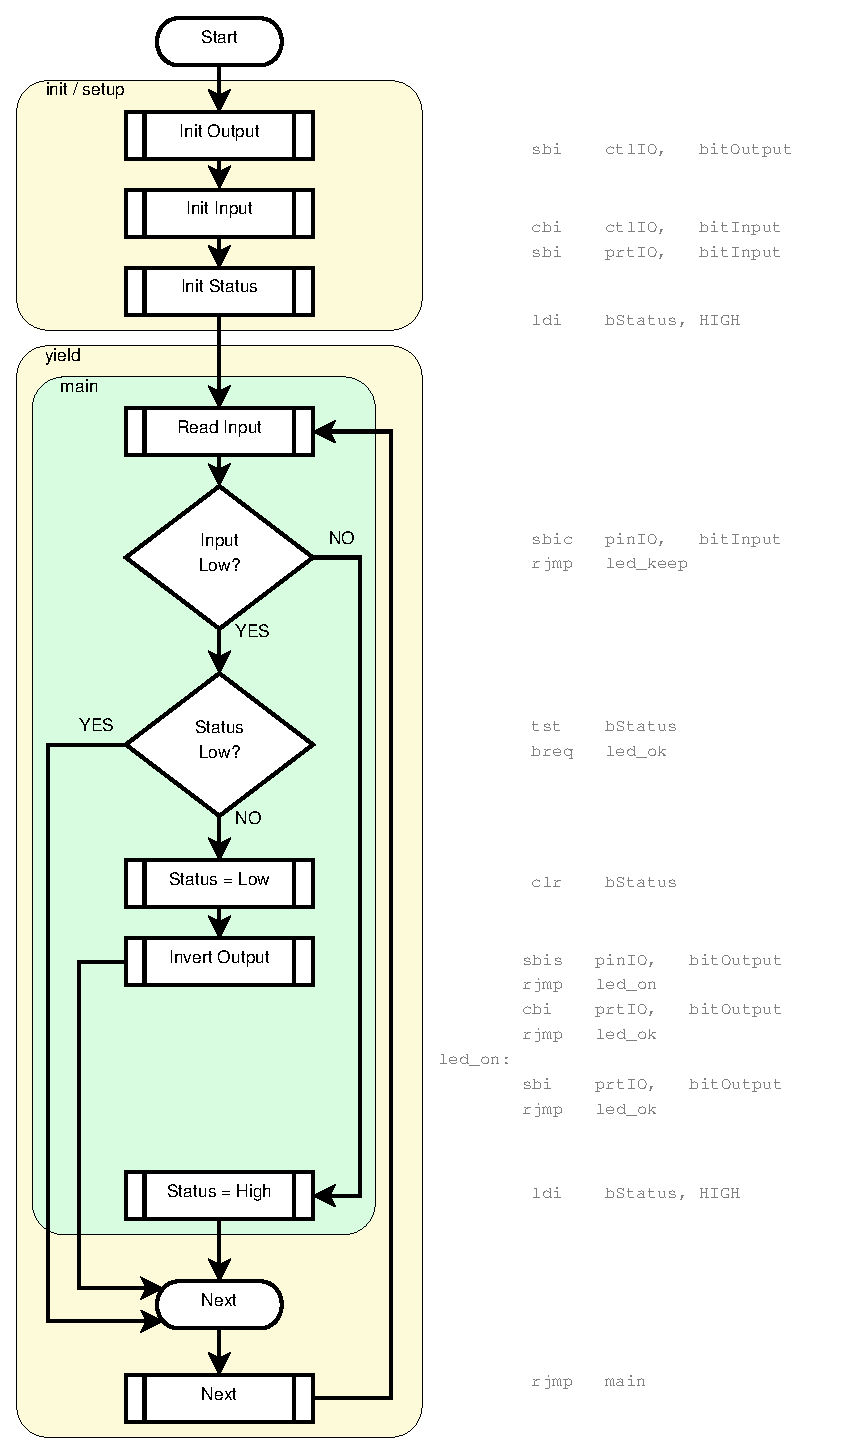
\includegraphics[height=210mm]{LED/S005_stable-decisions+symbols.eps}
!en   \caption{Stable Decisions - Flow Diagram}
!de   \caption{Stabile Entscheidungen - Ablaufplan}
  \label{S005FlowDiagam}
\end{figure}



!en X

!de Der grösster Störfaktor in der Informatik ist bekanntlich der Anwender. Nicht nur, dass seine Erwartungen von den Konzepten der Entwickler abweichen, es beginnt schon damit, dass er, in seinem Aufbau als Bioeinheit, unvorstellbar langsam ist. Die unglaubliche Langsamkeit des Anwenders ist ein technisches Problem, die Erwartungshaltung an die Art wie Geräte funktionieren ein ökonomisches. Wenn der gemeine Anwender unser Gerät nicht akzeptiert, wird er es nicht kaufen und wir haben nichts zu essen.



!en \subsubsection{Slow users}
!de \subsubsection{Die unglaubliche Langsamkeit des Anwenders}



!en X

!de Eine Bioeinheit drückt einen Knopf und unser Gerät hat zu reagieren. Dummer Weise prüft unser Gerät den Schalter vielleicht 1.000.000 Mal in jeder Sekunde. Ein Mensch z.B. mag einen Knopf sehr schnell drücken und den Kontakt im Schalter für 0.2s schliessen. Unser Gerät erkennt während dessen 200.000 Mal, dass der Schalter durchgeschaltet ist. Dies wohlgemerkt bei einem ganz schnellen Menschen. Was der Mensch aber erwartet ist:

\begin{center}
!en Change the light ones as I press (in my view) the button ones!
!de Schalte das Licht einmal um wenn ich (aus meiner Sicht) den Knopf einmal drücke. 
\end{center}



!en X

!de Das Gerät darf also nur einmal umschalten auch wenn es 200.000 Mal feststellt, dass der Knopf gedrückt ist. Aus diesem Grund verwendet unser Programm den Wechsel des Schaltzustandes um den Vorgang des Schaltens zu erkennen. Problematisch dabei ist, dass elektrische Schalter prellen. Das heisst, sie stellen den Kontakt nicht so her wie Nutzer es annehmen. Anstatt einmal einzuschalten, prallen die mechanischen Elemente beim Aufprall aufeinander voneinander ab und trennen die Verbindung wieder, um sie Millisekunden später wieder zu schliessen. Das kann sich unterschiedlich oft wiederholen. Wie das genau abläuft ist von unzähligen Faktoren abhängig. 



!en \subsubsection{Fast feedback}
!de \subsubsection{Schnelle Rückmeldung}

!en Our feedback device is the light we control. We have no display oder acoustic device to us as feedback but the very same object that goes to be controlled. User feedback therefore simply means to manipulate the status of the light. Even if its cool in movies to do anything without any visible feedback, real living bio entities require 'immediate feedback' for every action. Otherwise they run into problems.

!de Unser einziges Rückmeldegerät, dass dem 



\begin{figure}[htbp]
  \centering
  \includegraphics[width=120mm]{LED/S005_stable-decisions_ideal_signal.png}
  \caption{Stable Decisions - Signal Diagram}
  \label{S005SignalDiagam}
\end{figure}

Figure \ref{S005SignalDiagam} shows the signal we have to expect (idealised). You have to remember, that our micro controller reads the 'LOW' status of the signal 100.000 times or more often. We do not measure time! The natural timing unit in micro controllers is cycles. Read cycles, CPU cycles, sensor cycles. This is important to recognise especially because different clock frequencies and different voltage leads to different physical cycle durations. A program that measures a certain event by 1000 cycles will receive 2000 if the clock is doubled up.

Different clock frequencies lead to different CPU dependent cycles. Different voltage may lead to different sensor cycles, depending on the specification of the sensor in question and the characteristics of the signal to measure. Further, different voltage may lead to different absolute sensor signals, but this is another chapter.

The signal we need to recognise at the moment is the switch from HIGH to LOW and back again. The LOW level will stay for an undefined time / amount of measure cycles. What we have to focus on is the change of the signal!

To deal with this there are only two moments in all this 'endless' button down phase - between 't1' and 't2' - where it is applicable to really change the LEDs status. At the beginning, as the signal changes from HIGH to LOW (t1) or at the end, where the signal changes from LOW to HIGH again (t2).

To give the human who uses our device (the user) immediate feedback about success or failure of his action, we decide to use the first phase (t1) to do all the action. So we have a simple mission: If the signal is LOW now and was HIGH the last time we looked, we change the LEDs state. This satisfies also the endless LOW state of the input signal and the change from LOW to HIGH where we have to do nothing. Not even accidentally! This way, the human feels his request immediately answered, even if he is unable to comprehend on which grade immediately it real is answered.


\subsection{Finding the event}

To find the event the signal has gone to ground, we have to be aware of the status of the signal from the previous query cycle. Which is easy but expensive. We simply use a register to store the previous input status.

We simply have to check if the last seen status was HIGH as log as the current status is LOW. The status accumulator register follows the status of the input signal after being used to query the change event.

If the one moment we are waiting for passes, we invert the LED status. That's all


\subsection{And some modesty}

In respect of things to come, we have to be modest in our style. The 'endless loop' which keeps the micro controller running and waiting without going wild, will be used for some important things:

\begin{itemize}
  \item It mostly contains the main program
  \item It possibly consist of multiple parts
  \item It consist of an undefined amount of functional separate program parts
\end{itemize}

So we have to ensure, to don't make any shortcut back to the 'main' label. As there can only be one Highlander, there can only be one jump back to 'main'. This jump resides at the very end of the main sequence. Like this:

\begin{lstlisting}
main:

  A_begin:
            block     A or goto to end of block A
  A_end:

  B_begin:
            block     B or goto to end of block B
  B_end:

  C_begin:
            block     C or goto to end of block C
  C_end

mein_end:
            finalise
            rjmp      main
\end{lstlisting}

In our flow diagram one part has to reach the next part regardless of how the program is flowing. The rounded rectangle 'next' represents the central point behind our (currently) one part. This is the position where the next program part would follow in the same manner.

